\subsection{DIP}
\label{sec:algorithms:dip}

\begin{figure}
    \centering
    \begin{subfigure}[b]{0.50\textwidth}
        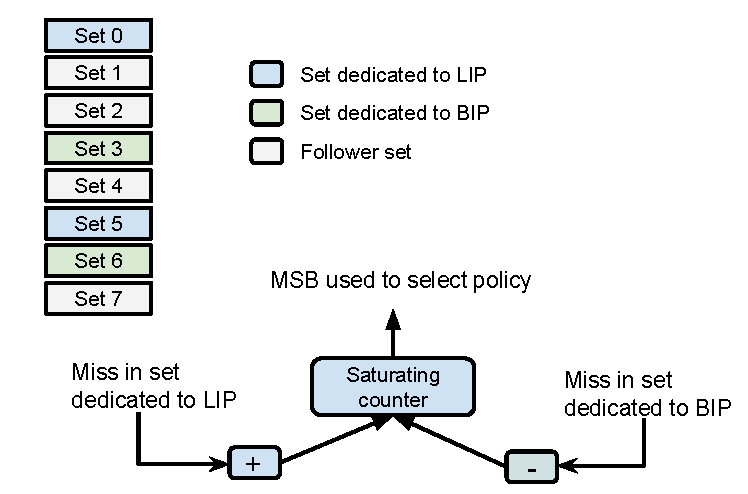
\includegraphics[width=\textwidth]{figures/algorithms/DIP_architecture}
        \caption{Set-dueling architecture.}
        \label{fig:algorithms:dip:set_dueling}
    \end{subfigure}    
    \begin{subfigure}[b]{0.45\textwidth}
        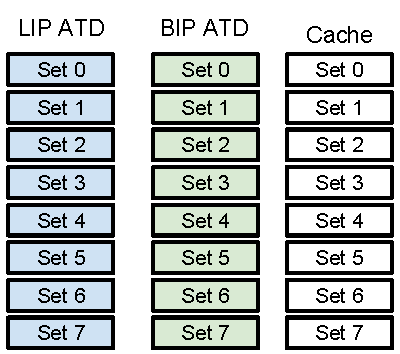
\includegraphics[width=.9\textwidth]{figures/algorithms/DIP_atd_architecture}
        \caption{ATD architecture.}
        \label{fig:algorithms:dip:atd}
    \end{subfigure}
    \caption{Alternate DIP organizations.}
\end{figure}

Dynamic Insertion Policy (DIP)~\cite{Qureshi2007} was originally proposed in 2007.
The DIP algorithm views the cache set as a stack, as in LRU.
Replacement and promotion policies are equal to LRU, DIP evicts the block at the LRU position, and following a cache hit a block moves to the MRU position.
In contrast to LRU, DIP is a combination of two insertion policies, the standard LRU insertion policy (LIP) and Binominal Insertion Policy (BIP).
LIP inserts new blocks at the MRU position.
BIP inserts new blocks either at the LRU position or with a small probability, $p = \frac{1}{32}$, at the MRU position. 
The overall DIP algorithm switches between the two insertion policies by always using the one that is expected to cause fewer cache misses.

By mostly inserting at the LRU position the BIP insertion policy can theoretically handle trashing memory access patterns.
When most new blocks enter at the LRU position, the upper parts of the LRU stack can contain blocks that have been re-referenced.
In a trashing access pattern, this results in part of the working set residing in the upper part of the stack while the rest are inserted at the LRU position and evicted at the next miss.
By sometimes inserting at the MRU position BIP will give blocks not referenced by the next miss a chance to stay in the cache. 
Inserting at the MRU position will also force stale cache blocks in the upper part of the stack to move towards the LRU position.

The authors of DIP present several methods to detect the best of the two replacement algorithm, one of them is set-dueling.
Set-dueling is implemented by having some sets of the cache always use BIP and some always use LIP.
A counter tracks the performance of the dueling sets.
Misses in LIP sets will increment the counter and misses in BIP sets will decrement the counter.
The most significant bit (MSB) of the counter can then be used to select the best performing of the two algorithms.
If the MSB is one, an overweight of misses in LIP sets are occurring, and BIP is the best performing algorithm. 
If the MSB is zero, then an overweight of BIP misses are occurring, and LIP is the best performing algorithm.
Figure~\ref{fig:algorithms:dip:set_dueling} shows the set dueling and algorithm selection architecture.
In the figure sets 0 and 5 are dueling sets for LIP while 3 and 6 are dueling sets for BIP.
All other sets are follower sets, meaning that they utilize the algorithm indicated by the selection logic.

Another solution is to utilize two Auxilliary Tag Directories (ATDs), as shown in Figure~\ref{fig:algorithms:dip:atd}.
An ATD is equal to the cache's tag directory; it keeps track of blocks present but does not store any data.
ATDs are, for this reason, cheaper than a full cache, but still requires more storage than dual-sets that use the existing cache.
As the figure shows, the two ATDs run one algorithm each and all operations on the main cache execute in parallel on the ATDs.
The same counter architecture controlled by misses in either ATD is used to select the best performing algorithm for the main cache.
The main advantage of using an ATD is that all available information is used when selecting between BIP and LIP.
Also, the entire cache will always use the best algorithm, where in set-dueling a fraction of the sets will always run the worst performing algorithm.
The difference between using an ATD and cache dueling sets in terms of misses were shown to be small in the original paper.
On their benchmarks, they measured an average decrease in misses by 22.3\% using ATDs, compared to a 21.3\% decrease when using 32 duel-sets~\cite{Qureshi2007}.

Figure~\ref{fig:algorithms:bip_example} shows an example cache set managed by DIP.
In the example, we assume BIP insertion with no insertions at the MRU position.
In the inital state, there are four blocks; A, B, C, and D.
A is at the MRU position and D is at the LRU position.
The first request is for C; this is a hit, and C is promoted to the MRU position, A and B are pushed towards the LRU position.
Then follows a request for E, which is a miss.
DIP evicts D at the LRU position and E is inserted in its place.
Then follows two requests to D; the first request is a miss causing E to be evicted and D to be inserted at the LRU position.
The second request is a hit and promotes D to MRU, pushing all other blocks one step towards the LRU position.

\begin{figure}[ht]
    \centering
    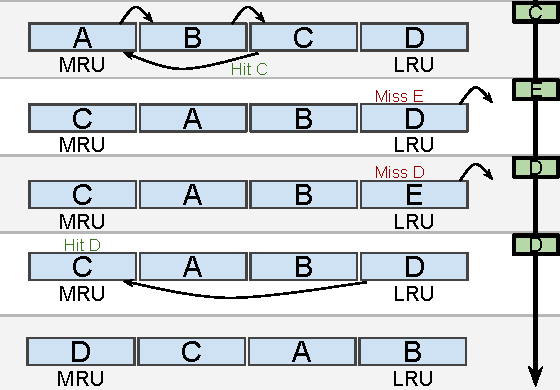
\includegraphics[width=.65\textwidth]{figures/algorithms/DIP}
    \caption[DIP managed 4-way cache set.]{DIP managed 4-way cache set. (Assuming BIP insertion)}
    \label{fig:algorithms:bip_example}
\end{figure}
